\section{Einleitung}
Die Anforderungsverwaltung (Requirements Management) wird nach dem International Requirements Engineering Board (IREB)  als einer der 4 Hauptaktivitäten im Requirements Engineering beschrieben.
% Pohl2015 S.5
Als zentrales Element steht hierbei die Sicherstellung der Verfolgbarkeit (auch: Nachvollziehbarkeit) von Anforderungen (Requirements Traceability). \cite{Pohl2015BasiswissenIREB-Standard}
% Pohl2015 S.130
Nach ISO/IEC/IEEE 29148:2011 ist eine Anforderung laut Pohl und Rupp verfolgbar,
\begin{quote}
[..] wenn sowohl der Ursprung der Anforderung als auch deren Umsetzung und die Beziehung zu anderen Dokumenten nachvollziehbar ist. \cite[S.48]{Pohl2015BasiswissenIREB-Standard}
\end{quote}
Eine so gepflegte Beziehung wird auch als Verfolgbarkeitsinformation bezeichnet. Ihre zentrale Rolle für das Requirements Management wird dadurch bestimmt, dass die Nutzung von Verfolgbarkeit allgemeine Techniken und Aspekte der Systementwicklung umfassend fördert und Vorraussetzung dafür ist, bestimmte Techniken im Entwicklungsprozess einsetzen zu können. \cite{Pohl2008RequirementsTechniken} Daher hat 
\begin{quote}
[d]ie Qualität der Nachvollziehbarkeit von Entwicklungsartefakten [..] einen großen Einfluss auf die Systementwicklung. \cite[S.507]{Pohl2008RequirementsTechniken}
\end{quote}
Die Sicherstellung der Qualität ist damit oberstes Gebot um Verfolgbarkeit gewinnbringend im Entwicklungsprozess einsetzen zu können. 

Was bedeutet aber der Begriff \enquote{Qualität} in der Requirements Traceability? Nach Gotel \& Finkelstein lässt sich Verfolgbarkeit in Pre-Requirements Specification (RS) und Post-Requirements Specification (RS) einteilen. 

\begin{figure}[!htb]
  \centering
  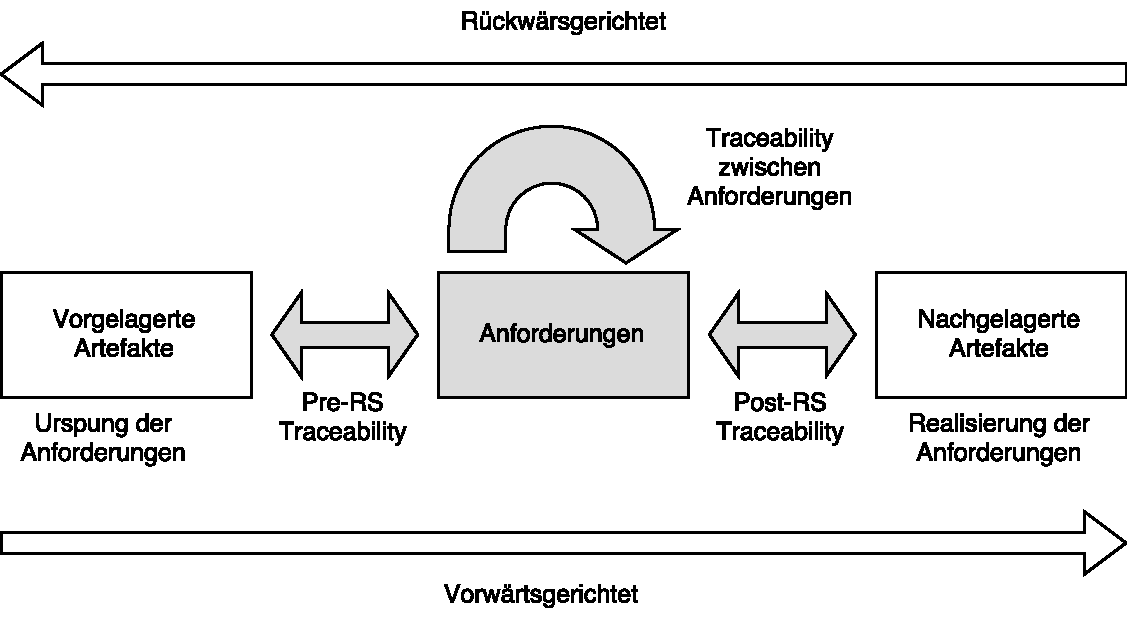
\includegraphics[width=3.4in]{PohlRupp2015_Fig_8_5.pdf}
  \caption{nach \cite[Fig. 8.5]{Pohl2015BasiswissenIREB-Standard}}
  \label{fig:abb1}
\end{figure}

Wie in \ref{fig:abb1} dargestellt wird zwischen drei Arten von Verfolgbarkeit unterschieden:

\begin{itemize}
    \item \textbf{Pre-RS:} Alle Beziehungen zu Artefakten die einer Anforderung vorgelagert sind z.B. Dokumente, Interviews etc. Im allgemeinen der Ursprung einer Anforderung
    \item \textbf{Post-RS:} Alle Beziehungen die einer Anforderung nachgelagert sind z.B Implementierung, Tests. Im allgemeinen die Auswirkung einer Anforderung
    \item \textbf{Verfolgbarkeit zwischen Anforderungen:} Abhängigkeiten oder Beziehungen zwischen Anforderungen. So kann z.B. eine Anforderung aus einem Konflikt zwischen zwei Anforderungen entstehen oder diese ersetzen. Im allgemeinen spricht man von einer Verfolgbarkeit über die Spezifikation \cite{Pohl2015BasiswissenIREB-Standard}.
\end{itemize}

Auf dem Pre-RS \& Post-RS Modell aufbauend, führt Pohl eine weitere Differenzierung ein, wie in \ref{fig:abb2} dargestellt.

\begin{figure}[!htb]
  \centering
  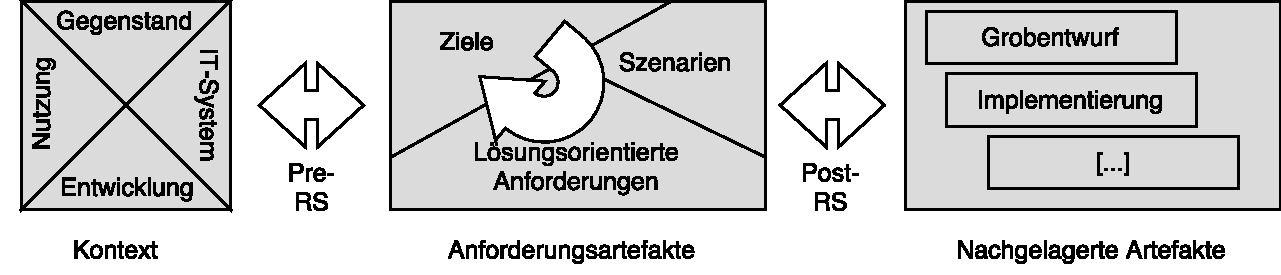
\includegraphics[width=3.4in]{Pohl2008_Fig_30_3.pdf}
  \caption{nach \cite[Fig. 30.3]{Pohl2008RequirementsTechniken}}
  \label{fig:abb2}
\end{figure}

Die \enquote{Erweiterte Pre- und Post-Traceability} präzisiert die Sicht auf die vor- und nach-gelagerten Artefakte. Die Pre-RS Traceability beschreibt alle Beziehungen zwischen Anforderungsartefakten und Aspekten in einer der 4 Sichten des Systemkontext. Die Post-RS Traceability beschreibt alle Beziehungen zwischen Anforderungsartefakten und nachgelagerten Artefakten die im Entwicklungsprozess entstehen. Die Beziehung zwischen Anforderungen umfasst zusätzlich die Verfolgbarkeit zwischen Zielen, Szenarien und lösungsorientierten Anforderungen \cite{Pohl2008RequirementsTechniken}.

Zusammenfassend lässt sich festhalten, das Requirements Traceability die Verfolgbarkeit einer Anforderung vom Ursprung bis zur Implementierung beschreibt. Diese Beziehung muss bidirektional sein, d.h. sie ist in vorwärts- wie in rückwärtsgerichteter Richtung möglich. Eine Verfolgbarkeit besteht dabei zwischen allen vor- und nach-gelagerten Artefakten im Entwicklungsprozess, wobei nach Pohl diese aus dem Kontext, Anforderungsartefakten und nachgelagerten Entwicklungsartefakten besteht. Die Qualität einer Verfolgbarkeit ist bestimmt durch die Vollständigkeit, Konsistenz und Fehlerfreiheit der Verfolgbarkeitsinformationen.

Die Erfassung ist jedoch ein manueller Prozess und dadurch fehleranfällig. Nach Walia \& Carver ist eine der Ursachen für Probleme im Requirements Engineering auf Inkonsistenzen in der Requirements Traceability zurückzuführen, die mitunter durch ein unzureichendes Requirements Management oder durch Fehler von Teammitgliedern verursacht werden \cite{Walia2009AErrors}. 

Um die Qualität sicherzustellen ist es wichtig zu wissen welche Probleme in der Requirements Tracebility existieren und welche Methoden es gibt um diese zu vermeiden.
Das können präventive sowie kurative Maßnahmen sein.

Als zentrales Ziel dieses Systematic Literature Review steht somit die

\enquote{Identifikation von Qualitätsproblemen in der Requirements Traceability, um sie frühzeitig erkennen und vermeiden zu können.

%In diesem Systematic Literature Review soll daher der aktuelle Forschungsstand zu Problemen im Management von Requirements Traceability und Maßnahmen ihrer Vermeidung näher beleuchtet werden.

%\section{Vorgehen}
%Zu Beginn wurde ein Systematic Literature Review (SLR) durchgeführt, um Probleme im Management von Requirements Traceability zu bestimmen, die die Qualität negativ beeinflussen. 